\chapter{Apoio à Docência}
\thispagestyle{empty}
\label{cap: apoioDocencia}
Neste capítulo, apresentaremos os principais recursos físicos e estruturais da \ac{GPF}, disponíveis aos docentes para melhor desempenharem suas atividades.

\section{Sala dos Professores}
\setlength\intextsep{0pt}
\begin{wrapfigure}[9]{r}{0.5\textwidth}
    \centering
    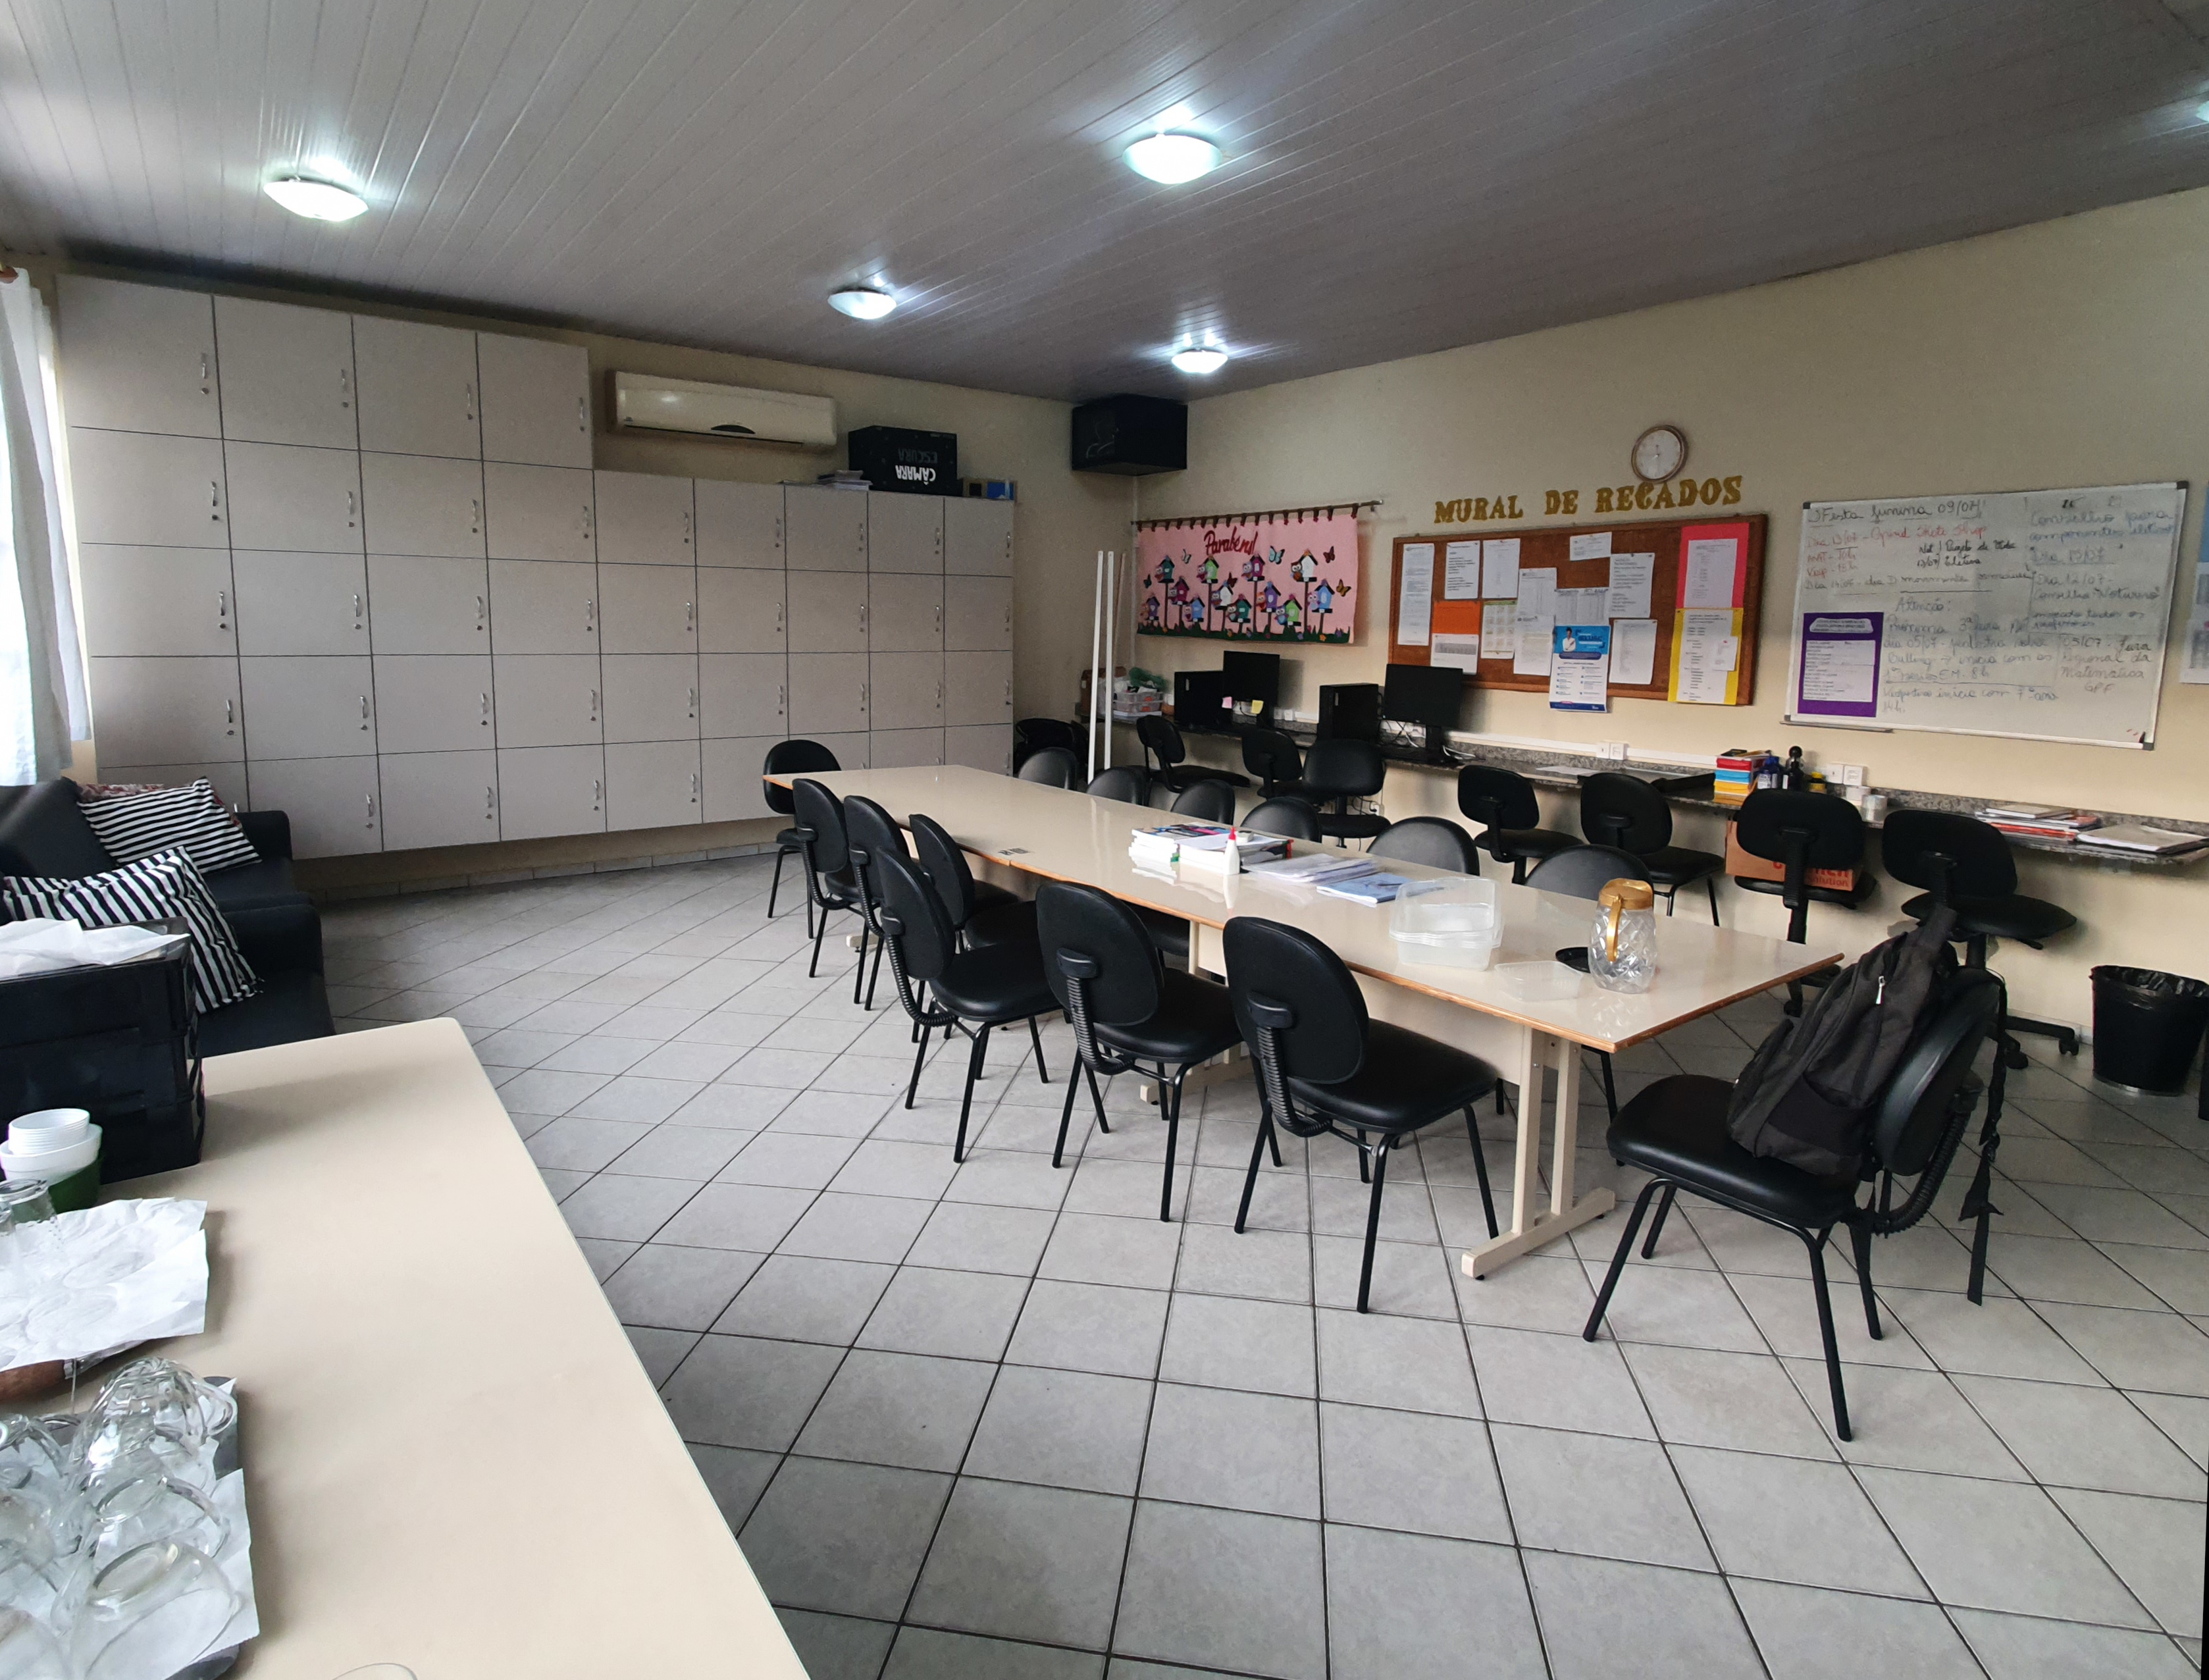
\includegraphics[width=.45\textwidth]{03-elementos/03.2_textual/03.2.1_fig/sala-de-profs01.jpg}
    \caption{Sala dos Professores}
    \label{fig:salaDosProfs}
\end{wrapfigure}
Bem espaçosa a Sala dos Professores, \autoref{fig:salaDosProfs}, possui: geladeira, forno de micro-ondas, aparelho de ar-condicionado e um purificador de água. É equipada com dois desktops conectados à internet. Cada professor tem um espaço nos armários e é nele que fica guardado o \emph{Data-Show} para uso em aulas diferenciadas.

\section{Laboratório}
As aulas experimentais podem ser conduzidas no Laboratório, preparado para atender as disciplinas de Física, Química e Biologia. Comporta cerca de 40 alunos e é composto por duas grandes bancadas e alguns armários. Há nele alguns materiais para conduzir experimentos de cinemática, física térmica e eletrostática, no entanto o professor da disciplina prefere usar a sala de aula para estas atividades.

\section{Laboratório de informática}
\setlength\intextsep{0pt}
\begin{wrapfigure}[7]{l}{0.45\textwidth}
    \centering
    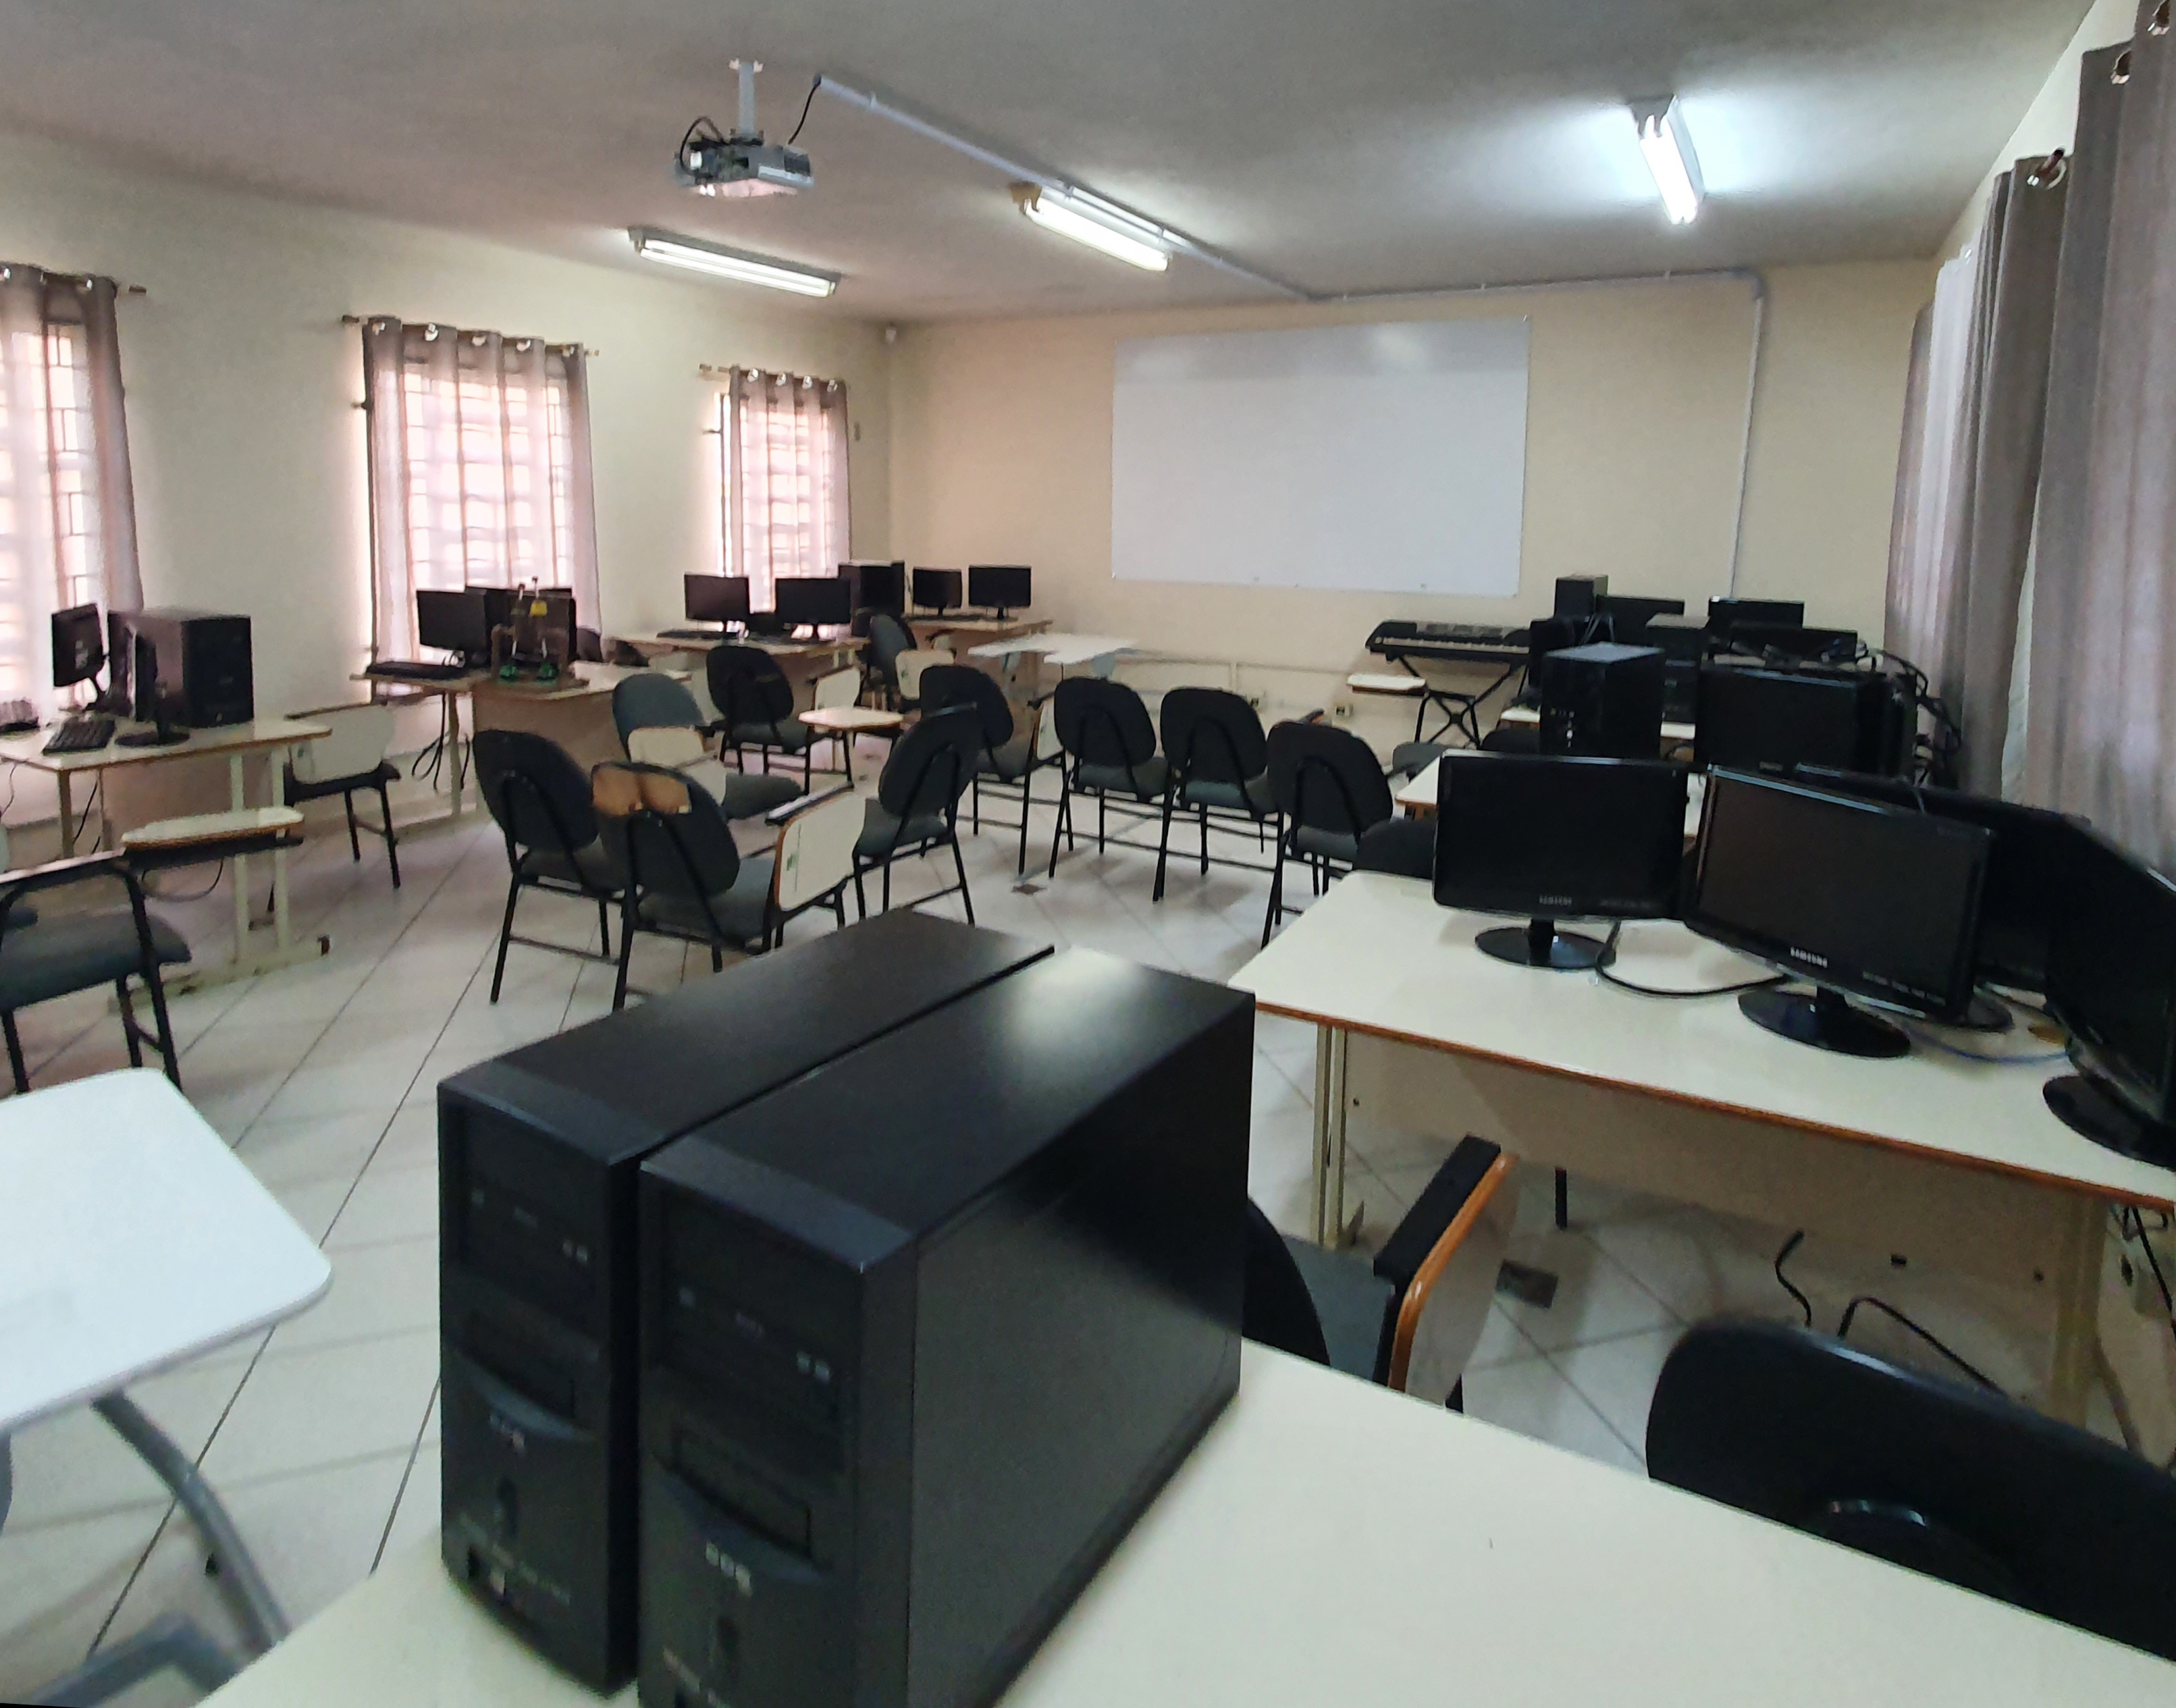
\includegraphics[width=.4\textwidth]{03-elementos/03.2_textual/03.2.1_fig/sala-de-informatica02.jpg} 
    \caption{Laboratório de informática}
    \label{fig:salaDeInformatica}  
\end{wrapfigure}
O Laboratório de Informática, \autoref{fig:salaDeInformatica}, é composto por nove desktops e dezenove monitores com acesso à internet, tem capacidade para atender até dezenove alunos em virtude da quantidade de dispositivos. Possui ainda uma Lousa Melamínica ($350\times 120$)\cm\; e retroprojetor.

\section{Salas de aula}
As Salas de Aulas são planejadas para comportar, em média, trinta alunos. Boa parte das salas possui aparelho de ar-condicionado, armários e são devidamente equipadas com Lousa Melamínica ($400\times 120$)\cm.

\section{Auditório}
\setlength\intextsep{0pt}
\begin{wrapfigure}[9]{r}{0.4\linewidth}
    \centering
    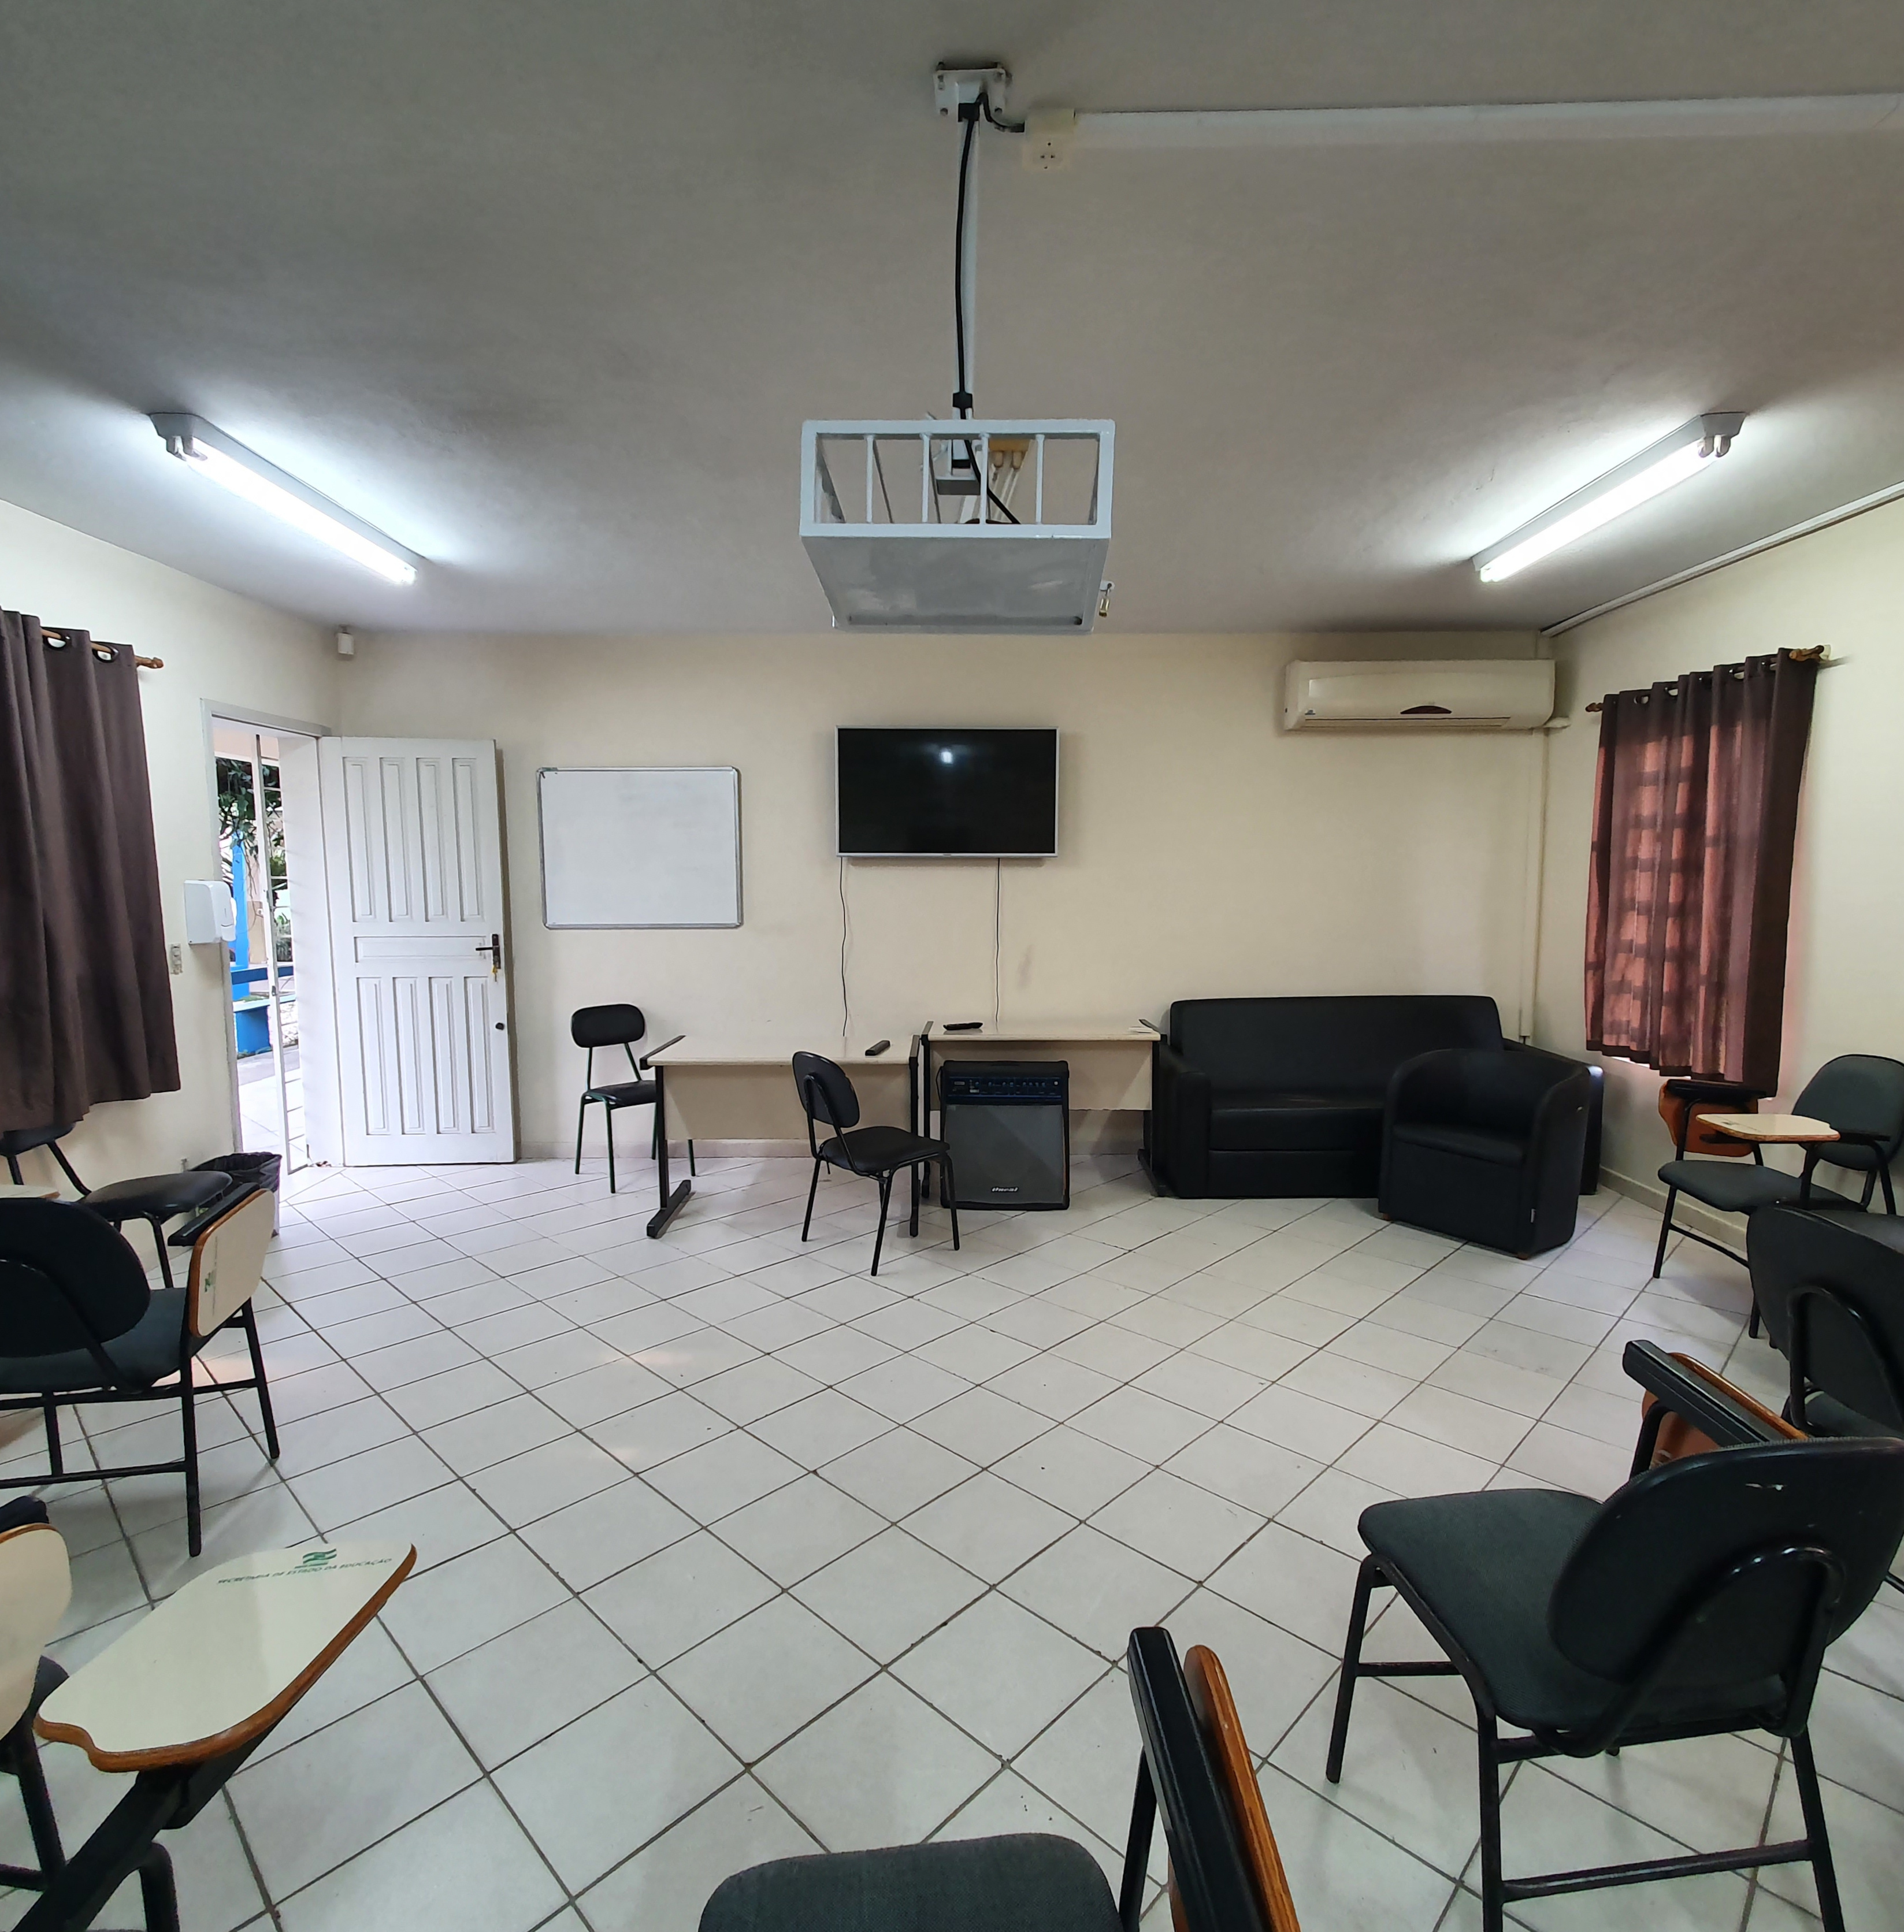
\includegraphics[width=.35\textwidth]{03-elementos/03.2_textual/03.2.1_fig/auditorio01.jpg} 
    \caption{Auditório}
    \label{fig:auditorio}    
\end{wrapfigure}
O auditório, \autoref{fig:auditorio}, tem capacidade para comportar um total quarenta pessoas e é equipado com um televisor de led $40\inch$, caixa de som amplificada multi-uso Oneal-OCM modelo 550 de $80\Watt$ de potência rms, um retroprojetor e ar-condicionado.

\section{Biblioteca}
No acervo da Biblioteca, \autoref{fig:biblioteca}, encontram-se livros didáticos de todas as disciplinas, livros de literatura nacional e internacional, almanaques, \acp{DVD} educativos, revistas de assuntos dos mais variados e jornais. Possui também uma televisão de $32\inch$ a tubo conectada à uma leitora de \ac{DVD}, mesas e cadeiras o suficiente para comportar uma pequena turma de 10 pessoas.
\vspace{8pt}

\begin{figure}[!ht]
    \begin{center}
        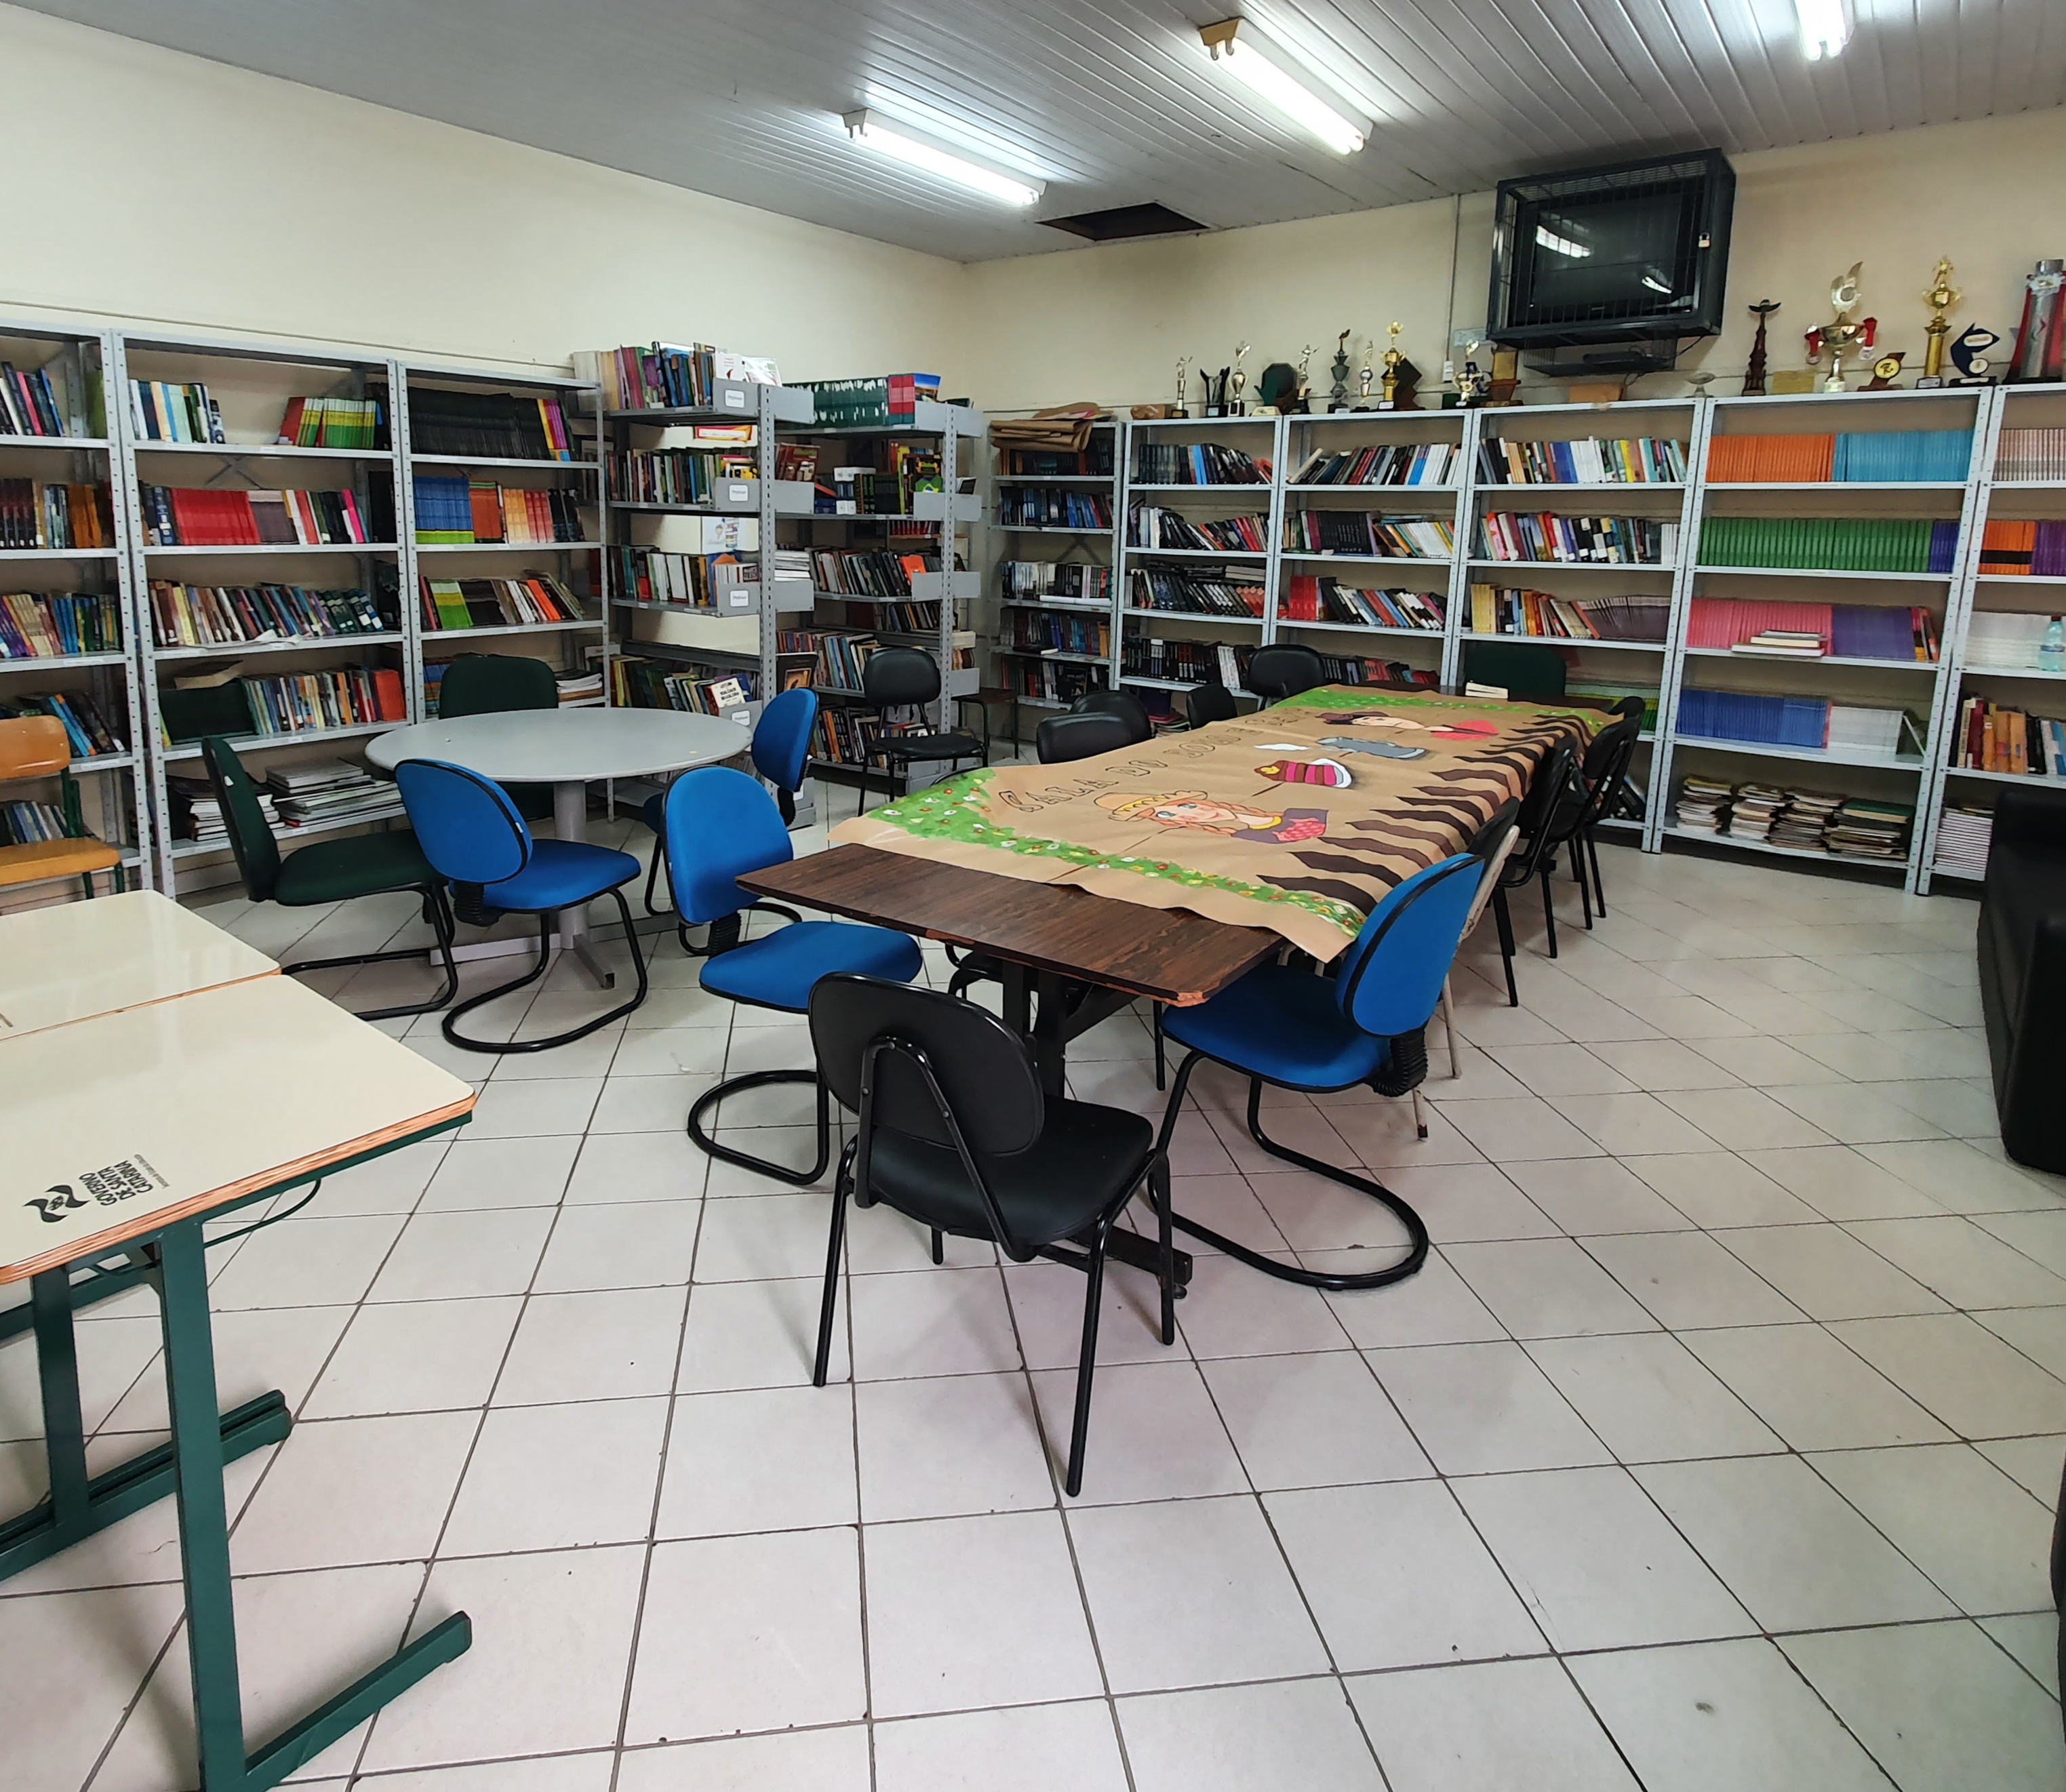
\includegraphics[width=.6\textwidth]{03-elementos/03.2_textual/03.2.1_fig/biblioteca01.jpg}
        \caption{Biblioteca}
        \label{fig:biblioteca} 
    \end{center}    
\end{figure}

%\newpage
\section{Outros Recursos}
\setlength\intextsep{0pt}
\begin{wrapfigure}[11]{l}{0.5\linewidth}
    \centering
    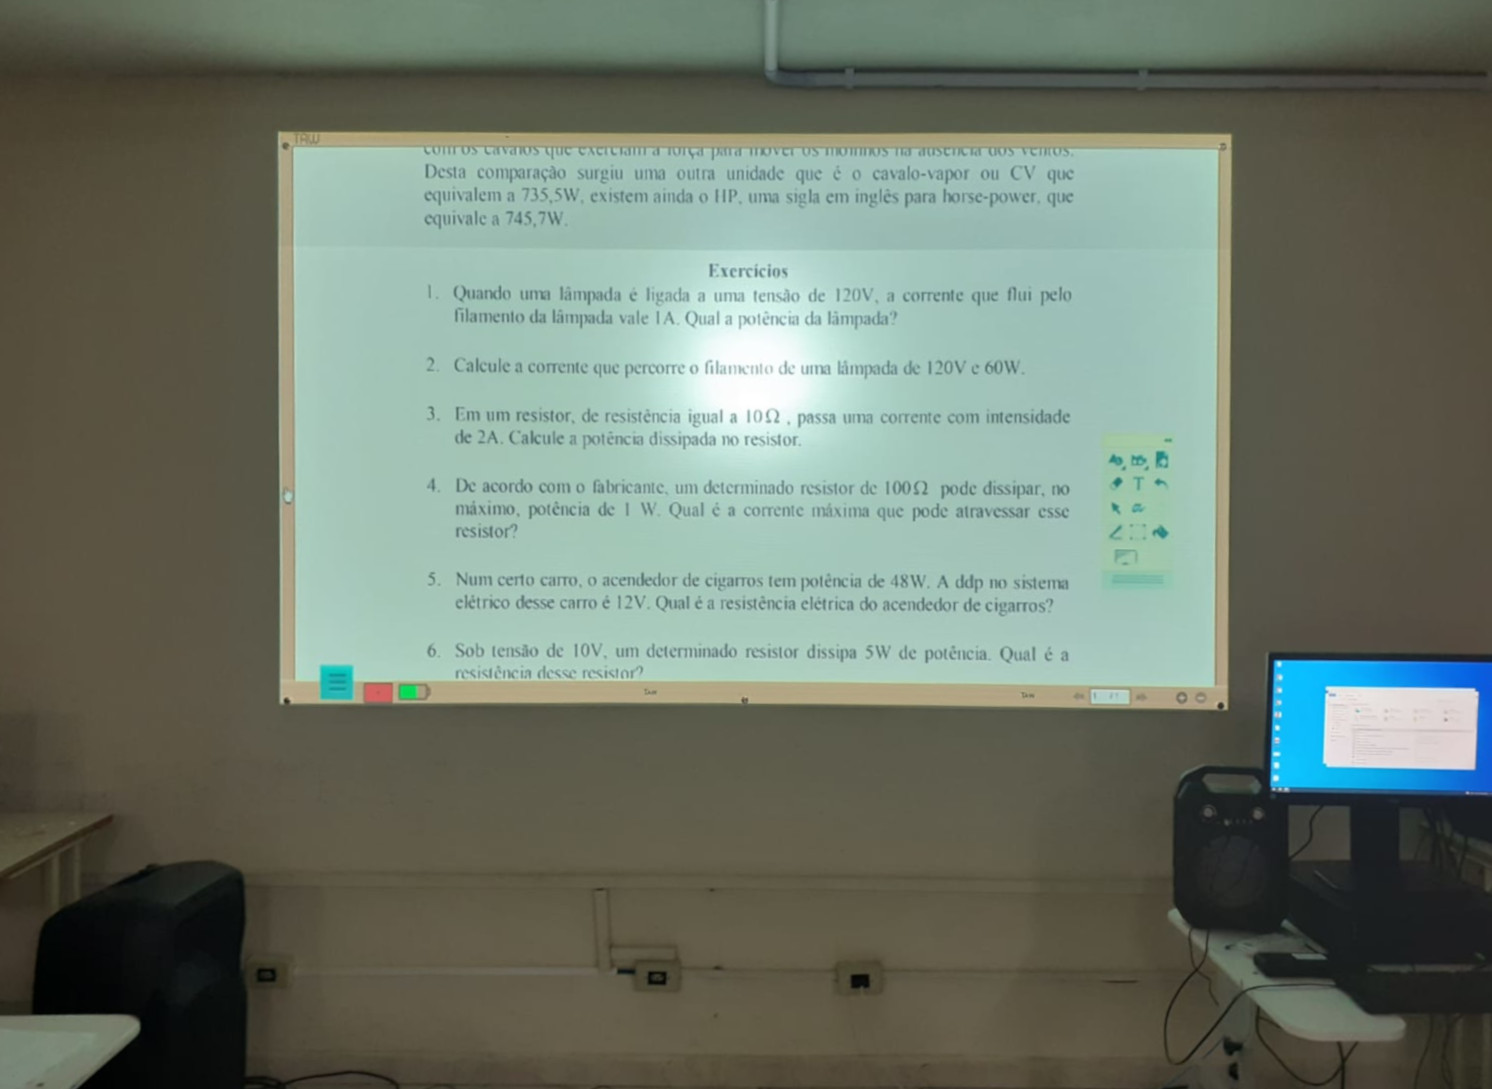
\includegraphics[width=.45\textwidth]{03-elementos/03.2_textual/03.2.1_fig/d-lousa.jpeg} 
    \caption{Lousa Digital}
    \label{fig:lousa-d}    
\end{wrapfigure}
Recentemente foi instalada uma lousa digital interativa em apenas uma sala de aula, \autoref{fig:lousa-d}, nela é possível mostrar simulações, vídeos, sons, GIFs etc. É um recurso que poucos professores utilizam no momento, por somente haver uma em toda a escola. A escola tem previsão de até o final do ano de 2023, todas as salas de aulas possuam o equipamento instalado. A lousa já possui todos os dispositivos necessários para o seu devido funcionamento, ficando a critério do professor a opção de levar ou não seu notebook ou que mais achar melhor para incrementar a aula.

\section{Tablets}
A unidade também possui 32 Tablets conectados à internet de 200 Mb e com o sistema operacional Android. Neles, o professor costuma usar o aplicativo \emph{Kahoot} em atividades diferenciadas. Para manter os tablets sempre com a bateria carregadas e prontos para uso, a escola utiliza o gabinete móvel de recarga, como pode ser visto na \autoref{fig:tablets}.
\begin{figure}[!ht]
\vspace{8pt}
    \begin{center}
        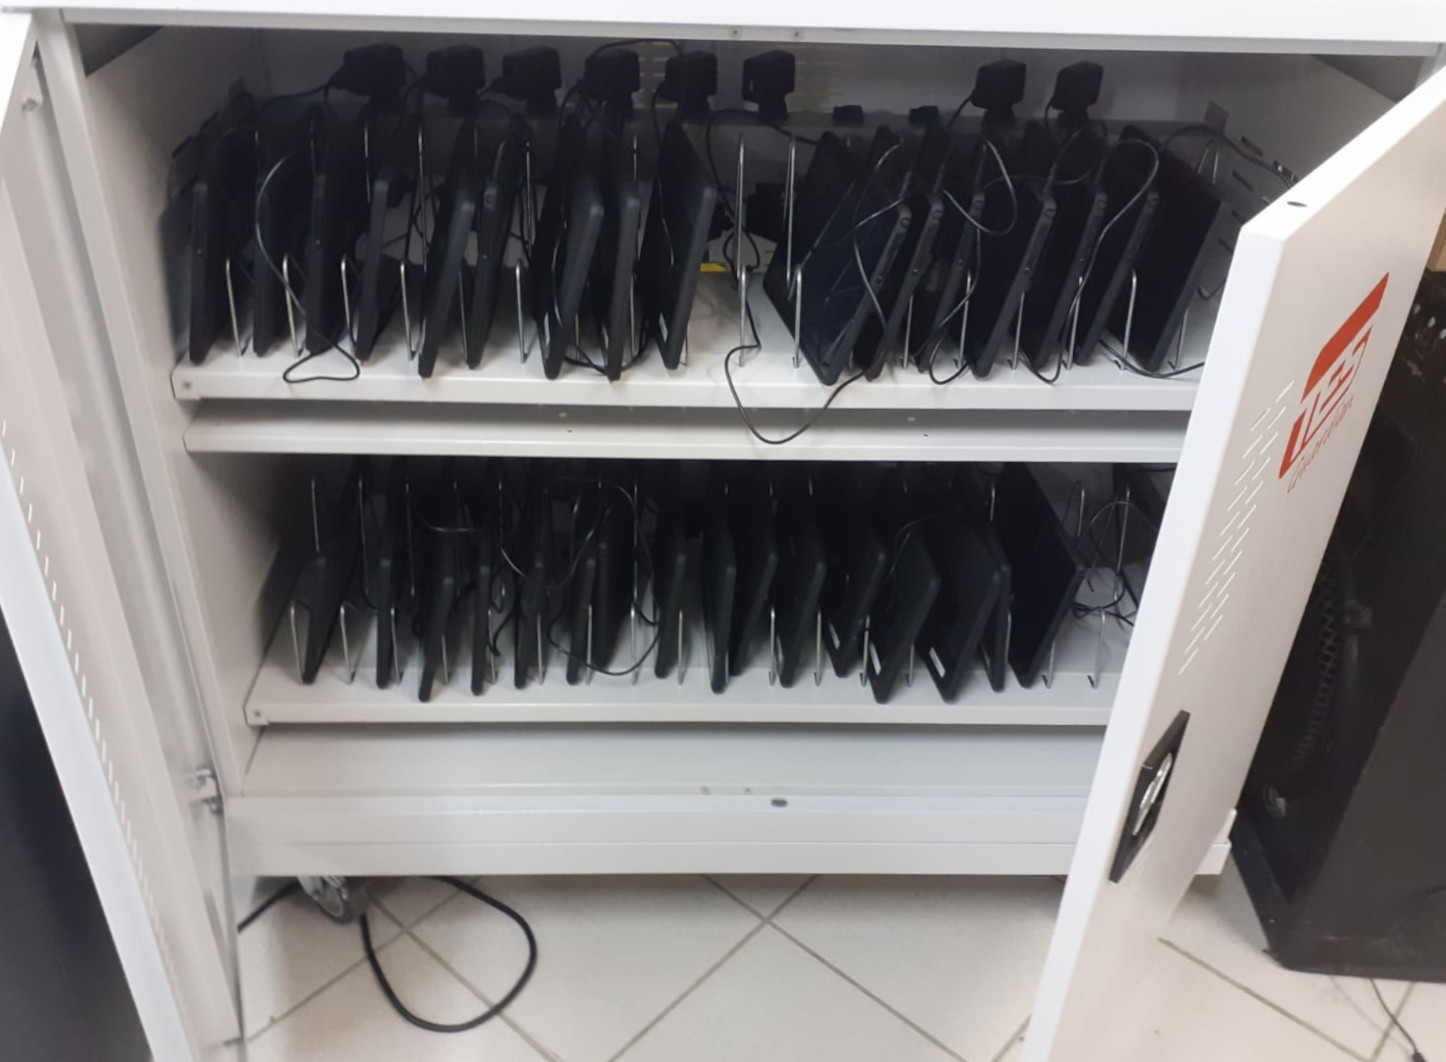
\includegraphics[width=.8\textwidth]{03-elementos/03.2_textual/03.2.1_fig/tablets.jpeg} 
        \caption{Tablets}
        \label{fig:tablets}    
    \end{center}
\end{figure}
